\subsubsection{Управление светодиодной лентой}

Для управления светодиодной лентой, необходима генерация ШИМ-сиг\-нала, подаваемая на контакт Din светодиодной ленты. Это, в свою очередь накладывает свои требования к генератору ШИМ-сигнала.

Для передачи информации, на контакт Din светодиодной ленты должны поступать последовательности по 24 бита, или по 3 байта, которые отвечают за цвет определённого светодиода. При модуляции используются длительности импульсов, согласно таблице~\ref{tab:ws2812__data_transfer_time}~\cite{Worldseim}.

\begin{table}[H]
  \caption{Длительность импульсов для управления светодиодом WS2812b}
  \label{tab:ws2812__data_transfer_time}
  \begin{tabular}{|c|l|c|}
  \hline
  \textbf{Обозначение} & \multicolumn{1}{c|}{\textbf{Описание}} & \textbf{Время} \\ \hline
  T0H                  & код "0", время высокого уровня         & 0,35 мкс       \\ \hline
  T1H                  & код "1", время высокого уровня         & 0,9 мкс        \\ \hline
  T0L                  & код "0", время низкого уровня          & 0,9 мкс        \\ \hline
  T1L                  & код "1", время низкого уровня          & 0,35 мкс       \\ \hline
  RES                  & время низкого уровня                   & 50 мкс         \\ \hline
  \end{tabular}
\end{table}

Визуально ШИМ импульсы представлены на рисунке~\ref{img:WS2812__PWM_codes}.

\begin{figure}[H]
  \centering
  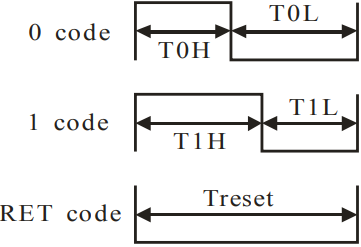
\includegraphics[height=0.2\textheight]{assets/images/practical/PWM__codes.png}
  \caption{ШИМ импульсы для управления WS2812b}
  \label{img:WS2812__PWM_codes}
\end{figure}

При кодировании цвета светодиода, последовательность из 24 бит представляется как 3 подряд идущих пакета, описывающих определённый основной сигнал. Первый пакет описывает зелёную составляющую цвета, второй -- красную, третий -- синюю. Биты в пакетах идут от старшего к младшему.

Например, для описания цвета, представленного в RGB как (18, 88, 160), необходимо преобразовать его в GRB, (88, 18, 160). Затем перевести их в двоичный вид, 01011000 00010010 10100000, и подать на вход Din светодиодной ленты в ШИМ. Для данного примера, ШИМ будет выглядеть как на рисунке~\ref{img:WS2812__PWM_example}.

\begin{figure}[H]
  \centering
  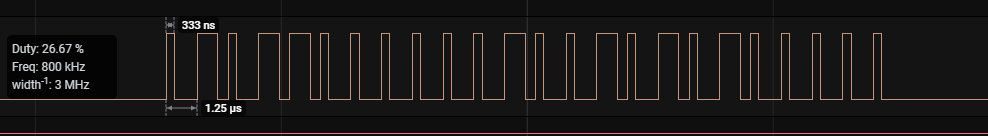
\includegraphics[width=0.9\textwidth]{assets/images/practical/PWM__example.jpg}
  \caption{Пример ШИМ для кодирования цвета}
  \label{img:WS2812__PWM_example}
\end{figure}

Для управления адресными светодиодными лентами с помощью языка программирования Node, выбранного в качестве основного для разработки серверной составляющей комплекса, наибольшей популярностью обладают 3 пакета~\cite{npm}:

\begin{itemize}
  \item node-pixel;
  \item rpi-ws281x;
  \item rpi-ws281x-native.
\end{itemize}

Node-pixel является наиболее популярным пакетом, но он также является самым <<тяжёлым>> пакетом и предполагает использование какой-либо другой платы, например, Arduino Nano, с помощью которой происходит управление светодиодной лентой. В этом случае Raspberry Pi выполняет роль интерпретатора языка Node, а плата, принимая полученные по I2C-шине данные, управляет светодиодной лентой. Данный пакет не был использован в проекте, так как его возможности излишни.

Rpi-ws281x и rpi-ws281x-native являются пакетами, близкими по популярности и предоставляемым способам управления светодиодными лентами. Они предоставляют возможность прямого управления светодиодной лентой с RPI, без использования каких-либо промежуточных контроллеров.

При разработке программной составляющей проекта был использован пакет rpi-ws281x-native, ввиду более подробной документации и использования при выполнении нативных привязок GPIO.

При работе с модулем rpi-ws281x-native для инициализации объекта управления светодиодной лентой, необходимо указать следующие параметры:

\begin{itemize}
  \item count -- количество светодиодов в ленте;
  \item gpio -- выход GPIO, к которому подключена лента. По умолчанию управление происходит с помощью GPIO18;
  \item invert -- изменение выходного сигнала. Применяется, если используется логический преобразователь уровней. По умолчанию значение false;
  \item brightness -- яркость, применяемая ко всем светодиодам в ленте. По умолчанию максимальна, 255;
  \item stripType -- тип светодиодов в ленте. По умолчанию WS2812.
\end{itemize}

Данные о ленте хранятся в виде массива чисел, где каждому элементу массива соответствует определённый светодиод. Обращение к светодиодам происходит по индексам.

Для отправления необходимого состояния на светодиодную ленту, используется метод render().

Перед тем, как завершить работу с лентой, необходимо очистить данные, хранящиеся на контроллерах её светодиодов. Это можно сделать с помощью метода reset(), который очистит данные на контроллерах светодиодов, и finalize(), который отключает драйвер управления светодиодной лентой и высвобождает ресурсы.

Например, в листинге~\ref{lst:node__rainbow} представлен скрипт, который запускает анимацию переливания цветов для всей светодиодной ленты.

\lstinputlisting[style=ES6, caption={Пример скрипта, запускающего анимацию переливания цветов на светодиодной ленте}, label={lst:node__rainbow}, linerange={19-29, 33-48}, consecutivenumbers=true]{assets/listings/practical/rainbow.js}

Пример работы эффекта переливания представлен на рисунке~\ref{img:ws2812__rainbow}.

\begin{figure}[H]
  \centering
  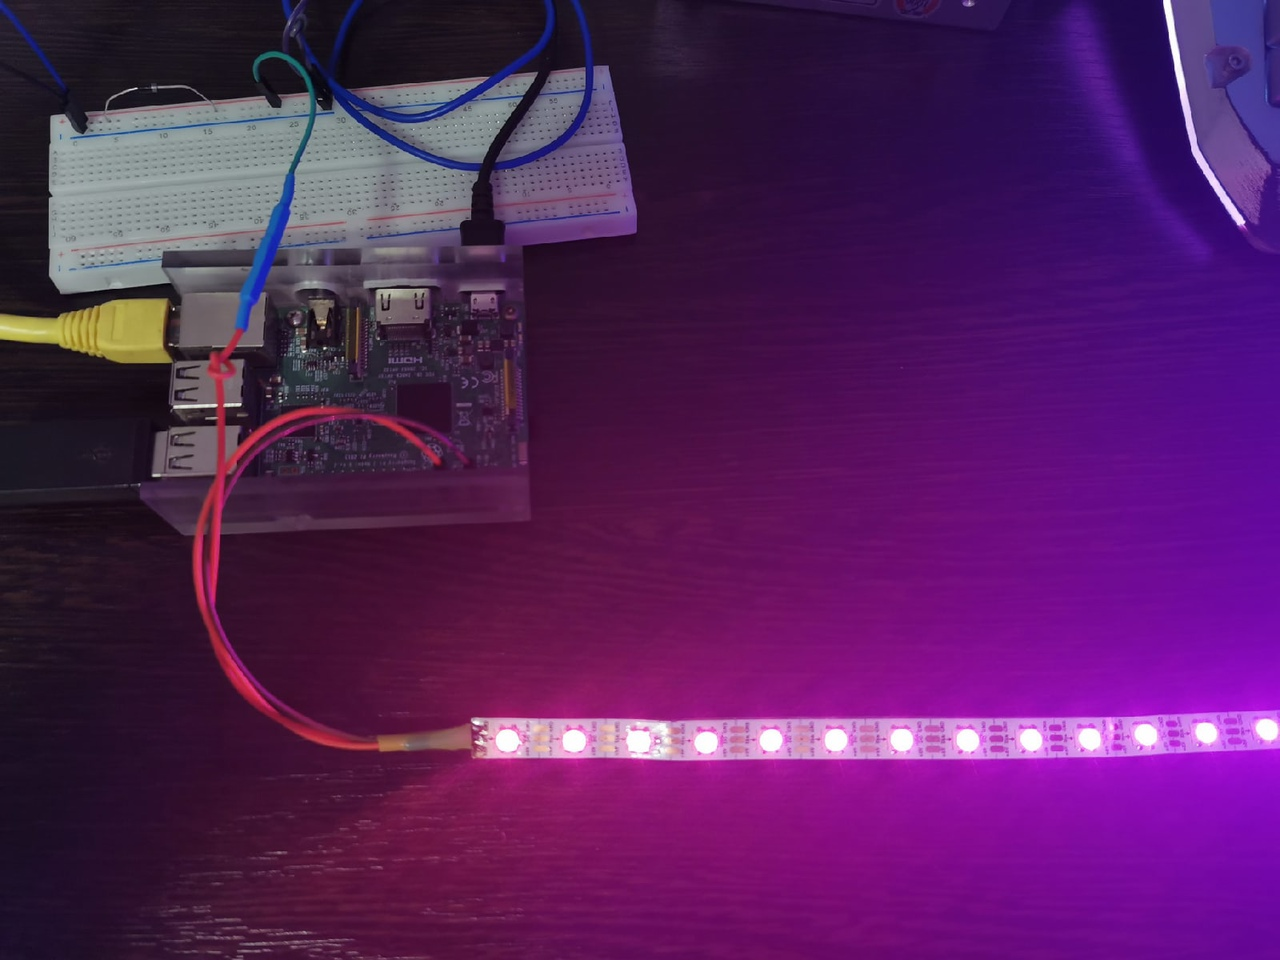
\includegraphics[width=0.9\textwidth]{assets/images/practical/Эффект переливания.jpg}
  \caption{Эффект переливания}
  \label{img:ws2812__rainbow}
\end{figure}

В случае, если необходимо, чтобы цвета выходили из центра светодиодной ленты и расходились в стороны, тогда скрипт будет выглядеть, как показано в листинге~\ref{lst:node__shift}. Предполагается, что число светодиодов в ленте чётное.

\lstinputlisting[style=ES6, caption={Пример функции, запускающего анимацию выхода цвета из центра светодиодной ленты в стороны}, label={lst:node__shift}, linerange={29-45}, consecutivenumbers=true]{assets/listings/practical/Server/LED.js}

Пример работы эффекта выхода цветов из середины ленты представлен на рисунке~\ref{img:ws2812__shift}.

\begin{figure}[H]
  \centering
  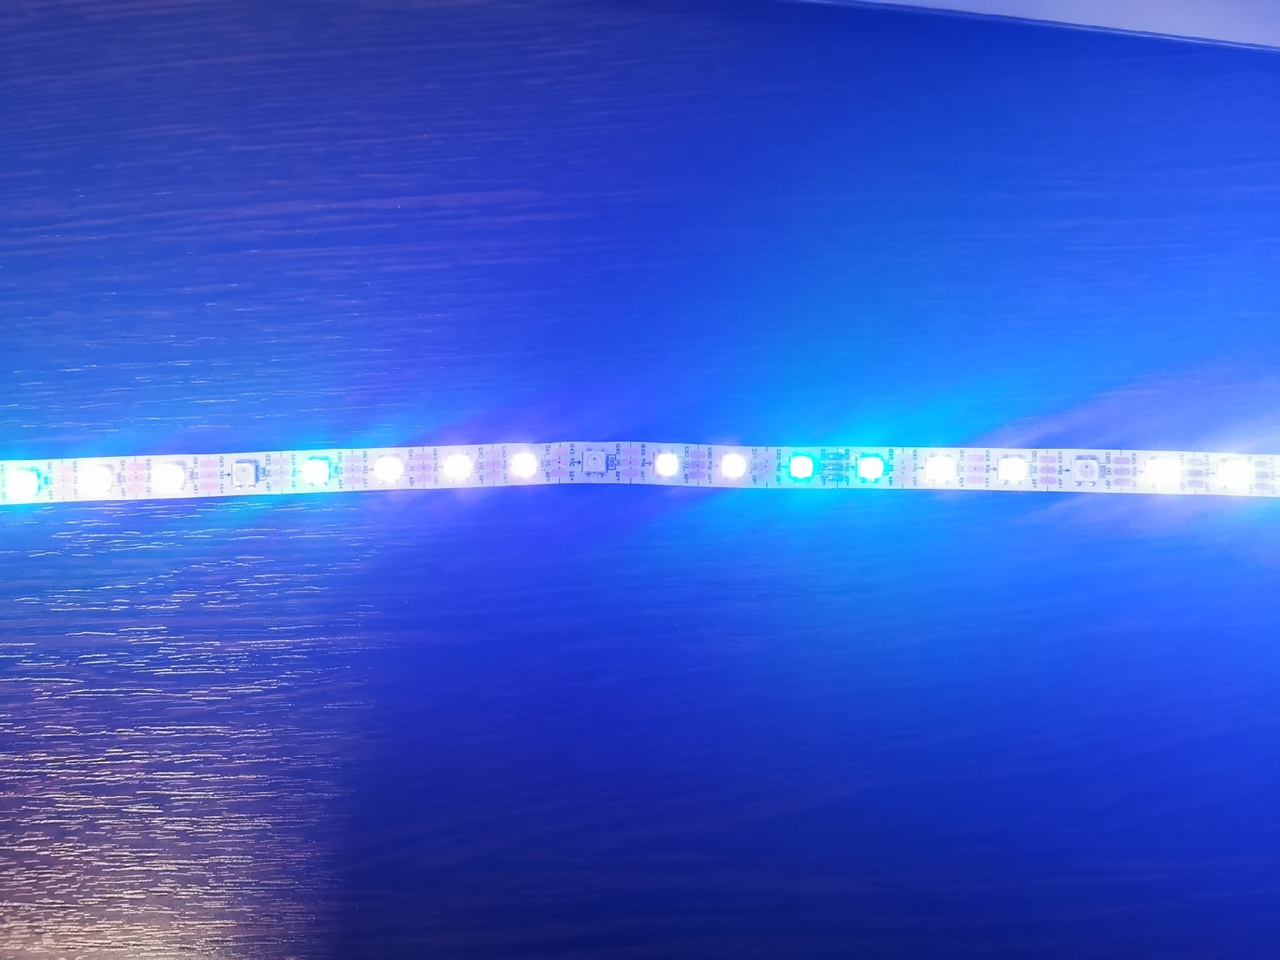
\includegraphics[width=0.9\textwidth]{assets/images/practical/Эффект из центра.jpg}
  \caption{Эффект выхода цветов из середины ленты}
  \label{img:ws2812__shift}
\end{figure}

В этой функции на вход поступают массив, описывающий светодиоды в ленте, и новый цвет, который необходимо отобразить начиная с центра. Сначала находится индекс центрального элемента, затем смещаются на один влево/вправо цвета светодиодов, и добавляется новый цвет. Возвращаемым значением является новое состояние светодиодной ленты.

Для отображения полученного состояния на светодиодной ленте, можно воспользоваться функцией, предложенной в листинге~\ref{lst:node__render}.

\lstinputlisting[style=ES6, caption={Пример функции отображения нового состояния светодиодной ленты}, label={lst:node__render}, linerange={107-113}, consecutivenumbers=true]{assets/listings/practical/Server/LED.js}

Полный код управления светодиодной лентой представлен в приложении~\ref{lst:LED__ALL}.